\begin{frame}[parent={cmap:software-testing-foundations}, hasprev=false, hasnext=true]
\frametitle{Técnica de teste}
\label{concept:test-technique}

\begin{block:concept}{Definição}
Técnica de testes são tipos de teste definidos de acordo com a fonte de informação utilizada para efetuar o teste de atividade.
\end{block:concept}

\begin{block:fact}{Técnica de testes and critério de teste}
\begin{itemize}
    \item Cada técnica de teste tem um conjunto de critérios de teste associado a ele.
\end{itemize}
\end{block:fact}
\end{frame}



\begin{frame}[hasprev=true, hasnext=true]
\frametitle{Técnica de teste}

\begin{block:fact}{Técnicas de teste de software}
\begin{itemize}
	\item Teste exaustivo;

	\item Teste aleatório;

	\item Teste particionado:
	\begin{itemize}
		\item Teste baseado em erro;

		\item Teste funcional;

		\item Teste estrutural;
	\end{itemize}
\end{itemize}
\end{block:fact}
\end{frame}



\begin{frame}
\frametitle{Técnica de teste}
\framesubtitle{Teste exaustivo}
\label{concept:exhaustive-testing}

\begin{block:concept}{Definição}
Um teste exaustivo executa o software com todo os possíveis valores de seu domínio de entrada.
\end{block:concept}

\begin{block:fact}{}
    \centering
    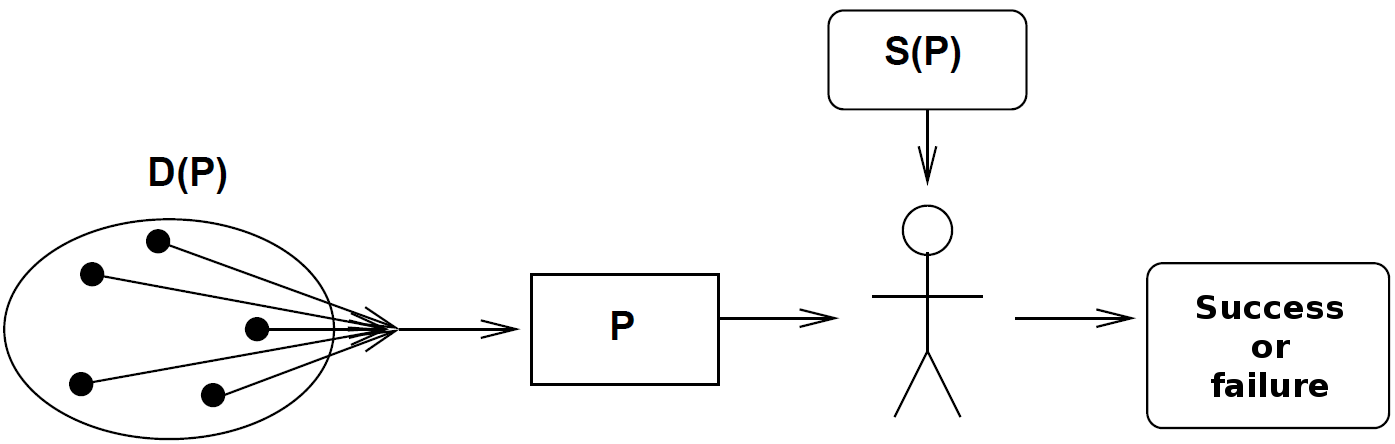
\includegraphics[width=\textwidth]{teste-de-software/conceitos-basicos/Imagens/exhaustive-software-testing}
\end{block:fact}

\hfill
\refie{example:blech-exhaustive-testing}{\beamerbutton{Example: Teste exaustivo of the blech function}}
\end{frame}



\begin{frame}
\frametitle{Técnica de teste}
\framesubtitle{Teste exaustivo}

\begin{block:fact}{Limitação do teste exaustivo}
\begin{itemize}
	\item Pode ser improveniente devivo ao tempo e ao custo de restrição, não para entrada de domínio finita, mas para grandes entradas;

	\item Impossível se o domínio de entrada é infinito;

	\item Em geral inviável.
\end{itemize}
\end{block:fact}
\end{frame}



\begin{frame}
\frametitle{Técnica de teste}
\framesubtitle{Teste aleatório}
\label{concept:random-testing}

\begin{block:concept}{Definição}
Teste aleatório utiliza um método sistemático para gerar casos de teste: requer modelar o espaço de entrada e, em seguida, os dados de amostra do espaço de entrada de forma aleatória.
\end{block:concept}

\begin{block:fact}{}
    \centering
    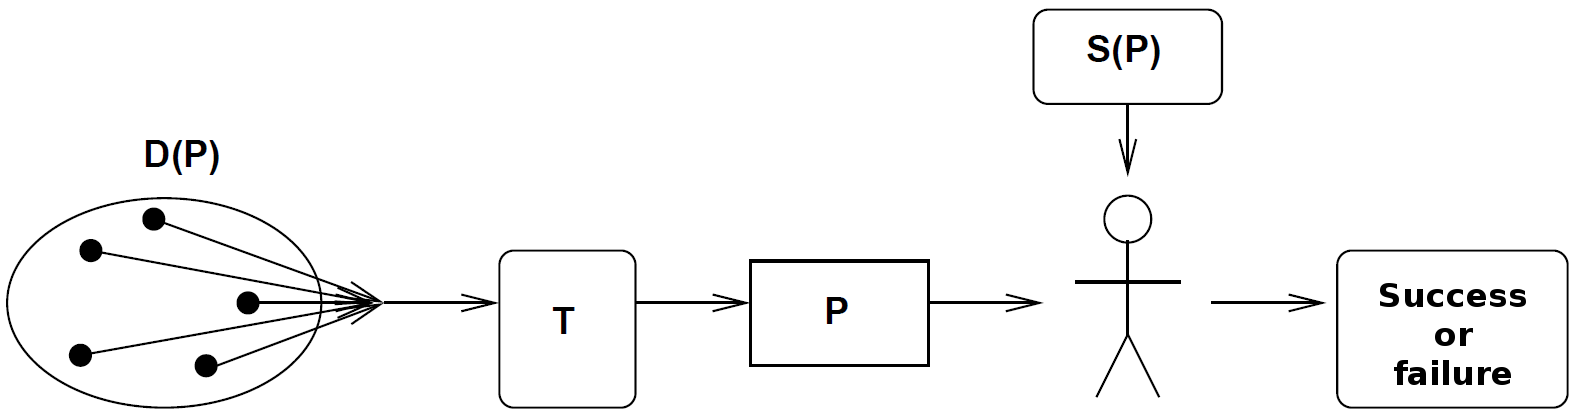
\includegraphics[width=\textwidth]{teste-de-software/conceitos-basicos/Imagens/random-software-testing}
\end{block:fact}
\end{frame}


\begin{frame}
\frametitle{Técnica de teste}
\framesubtitle{Teste aleatório}

\begin{block:concept}{Confiança}
\begin{itemize}
	\item Usando o teste aleatório, medidas estáticas de confiabilidade pode ser alcançada de acordo com um perfil operacional;

	\item Para cada (dados de entrada de um) caso de teste, é atribuída uma distribuição de probabilidade de acordo com a sua ocorrência na operação real.
\end{itemize}
\end{block:concept}

\begin{block:fact}{Eficácia}
\begin{itemize}
	\item Depende da definição do perfil operacional;

	\item Se a probabilidade de ocorrência de cada dado de entrada é o mesmo teste, o teste aleatório é considerado o teste menos eficaz para o teste de software~\cite[p. 43]{myers:2004}.
\end{itemize}

\end{block:fact}


\end{frame}


\begin{frame}
\frametitle{Técnica de teste}
\framesubtitle{Teste particionado}
\label{concept:partition-testing}

\begin{block:concept}{Definição}
Teste particionado entende-se como qualquer sistema de controle que obriga a execução de pelo menos um caso de teste a partir de cada subconjunto de uma partição do domínio de entrada.
\end{block:concept}

\begin{block:fact}{}
    \centering
    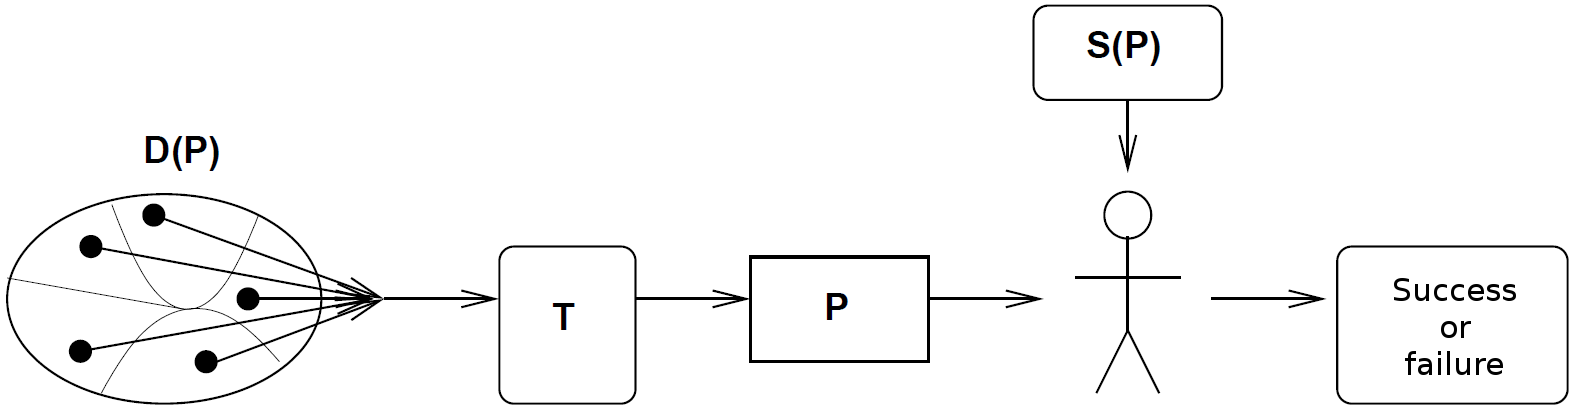
\includegraphics[width=\textwidth]{teste-de-software/conceitos-basicos/Imagens/partition-software-testing}
\end{block:fact}
\end{frame}



\begin{frame}
\frametitle{Técnica de teste}
\framesubtitle{Teste funcional}
\label{concept:functional-testing}

\begin{block:concept}{Definição}
Teste funcional é uma técnica baseada apenas nos requisitos e nas especificações.
\end{block:concept}

\begin{block:fact}{}
\begin{itemize}
	\item Teste funcional também é conhecido como teste da caixa preta;

	\item Teste funcional obtém requisitos de teste a partir da especificação de software:
	\begin{itemize}
		\item Teste funcional não requer nenhum conhecimento dos caminhos internos, a estrutura, ou a implementação do software em teste.
	\end{itemize}
\end{itemize}
\end{block:fact}

\hfill
\refie{example:functional-testing}{\beamerbutton{Example}}
\end{frame}


\begin{frame}
\frametitle{Técnica de teste}
\framesubtitle{Teste funcional}

\begin{block:fact}{Critério de teste funcional}
\begin{itemize}
	\item Partição de equivalência;
	\item Análise de valor limite;
	\item Gráfico de causa-efeito.
	\item \ldots
\end{itemize}
\end{block:fact}
\end{frame}



\begin{frame}
\frametitle{Técnica de teste}
\framesubtitle{Teste estrutural}

\begin{block:concept}{Definição}
Teste estrutural é uma técnica baseada nas partes internas, estrutura, e implementação do software em teste.
\end{block:concept}


\begin{block:fact}{}
\begin{itemize}
	\item Teste estrutural também é conhecido como caixa de teste branca;

	\item Teste estrutural consegue os requisitos de teste dos recursos de implementação.
\end{itemize}
\end{block:fact}

\begin{block:fact}{}
    \centering
    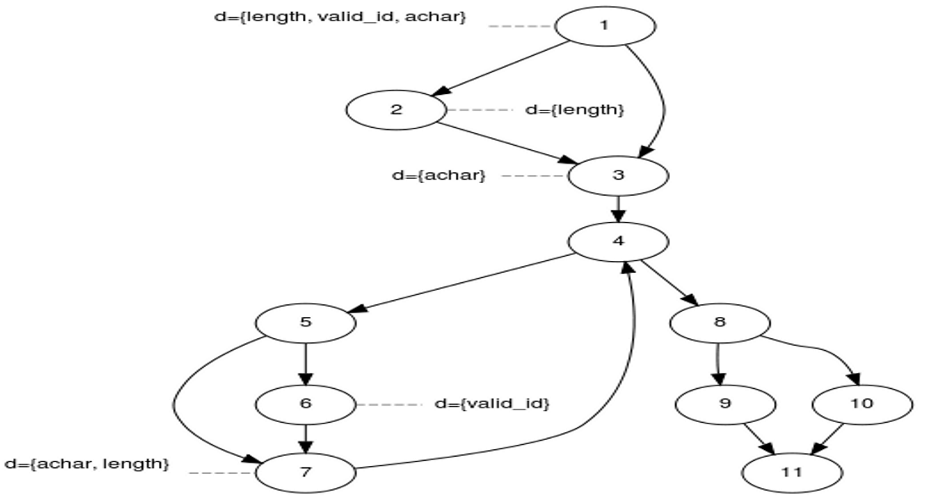
\includegraphics[width=6cm]{teste-de-software/conceitos-basicos/Imagens/structural-testing}
\end{block:fact}
\end{frame}


\begin{frame}
\frametitle{Técnica de teste}
\framesubtitle{Teste estrutural}
\label{concept:structural-testing-criteria}

\begin{block:fact}{Critérios baseados no controle de fluxo}
\begin{itemize}
	\item Critérios com base no fluxo de controle dentro de um programa:
	\begin{itemize}
		\item Cobertura de declaração;
		\item Cobertura de decisão;
		\item Cobertura de condição.
		\item \ldots
	\end{itemize}
\end{itemize}
\end{block:fact}


\begin{block:fact}{Critérios baseados no fluxo de dados}
\begin{itemize}
	\item Critérios baseados no uso de dados (criação de variável, definição e uso):
	\begin{itemize}
		\item Todas as utilizações;
		\item Todos potênciais uso;
		\item \ldots
	\end{itemize}
\end{itemize}
\end{block:fact}


\hfill
\refie{example:structural-testing}{\beamerbutton{Example}}
\end{frame}




\begin{frame}
\frametitle{Técnica de teste}
\framesubtitle{Teste baseado em erros}
\label{concept:fault-based-testing}

\begin{block:concept}{Definição}
Teste baseado em erros é uma técnica em que o teste é baseado em informações históricas sobre erros comuns detectados durante o ciclo de vida de desenvolvimento do software. 
\end{block:concept}

\begin{block:fact}{}
    \centering
    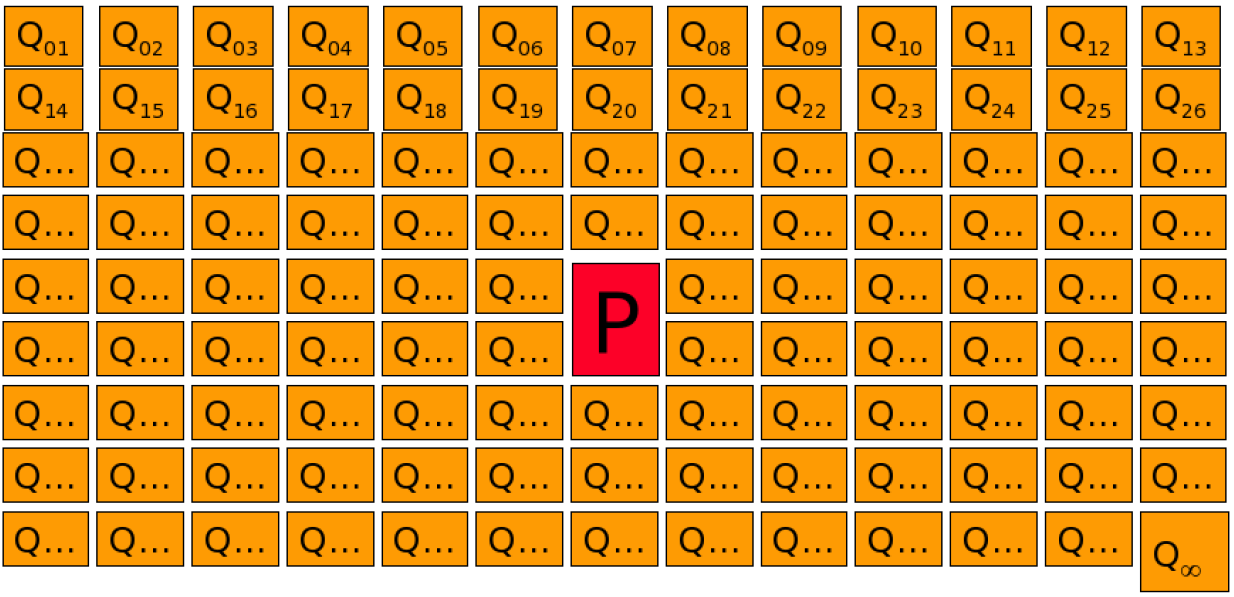
\includegraphics[width=7cm]{teste-de-software/conceitos-basicos/Imagens/mutation-testing}
\end{block:fact}
\end{frame}


\begin{frame}[hasprev=true, hasnext=false]
\frametitle{Técnica de teste}
\framesubtitle{Teste baseado em erros}
\label{concept:fault-based-test-criteria}

\begin{block:fact}{Critérios de teste baseado no erro}
\begin{itemize}
	\item Semeadura de erros.
	\item Mutação:
	\begin{itemize}
		\item Análise de mutantes;
		\item Mutação de interfaces.
		\item \ldots
	\end{itemize}
\end{itemize}
\end{block:fact}

\hfill
\refie{example:fault-based-testing}{\beamerbutton{Example}}
\end{frame}